\section{Handlers and algebraic effects}\label{sec:handlers-and-effects}
Algebraic effects and handlers have their foundation in category theory \cite{Plotkin2001a,Plotkin2013}. Plotkin and Power \cite{Plotkin2001b,Plotkin2001a} gave a categorical treatment of algebraic effects. The term ``algebraic'' implies that an effect ought to have an equational theory, however we consider only free algebras, that is our theories are equationless. Therefore we will not delve into the theoretical foundations of algebraic effects and handlers, rather we will take a more practical approach. Moreover, we will use the terms algebraic effect and effect interchangeably.

\subsection{Algebraic effect}
An algebraic effect is a collection of operation signatures \cite{Lindley2014}. For example, we might define an algebraic effect \type{Choice} for making a boolean choice with the following signature:
\[ \type{Choice} \defas \{ \type{Choose}: () \to \type{Bool} \} \]
Here \type{Choose} is a nullary operation whose return type is boolean. The effect \type{Choice} is the singleton set whose only member is \type{Choose}. 

The operation \type{Choose} is abstract, that is it has no concrete implementation. We say that computations composed from algebraic effects are \emph{abstract computations}. Without handlers abstract computations are meaningless as handlers faithfully interpret effects by instantiating them with concrete implementations. 

\subsection{Effect handler}
Benton and Kennedy generalised exception handlers \cite{Benton2001} (as known from SML, C\#, Java, etc) to expose a continuation to the programmer in the case no exceptions occurred during the handled context. Later their work was adapted by Plotkin and Pretnar \cite{Plotkin2013} to handle arbitrary effects, thus they coined the notion of handlers for algebraic effects.

Intuitively, an effect handler is a generalised function which takes an abstract computation as input, and embodies a collection of cases for pattern matching on operations that may be discharged during the evaluation of the input computation.

\subsection{Interpreting effects as computation trees}
Abstract computations are syntactic structure without a particular semantics. Handlers assign semantics to abstract computations.
To further develop intuition about handlers and effects we illustrate a diagrammatic interpretation of effects as computation trees \cite{Lindley2014}. Moreover, we see how we can assign different semantics to the same abstract computation. Consider the following expression:
\begin{lstlisting}[style=ocaml]
if Choose() then
  if Choose() then
    2
  else
    4
else
  if Choose() then
    8
  else
    16 
\end{lstlisting}
The expression is a nested conditional expression.
We can picture this expression as a tree where the nodes encode operations, edges correspond to branching, and the leaves encode concrete values. For example Figure \ref{fig:condexp} depicts the above expression as a computation tree.
\begin{figure}[H]
\begin{center}
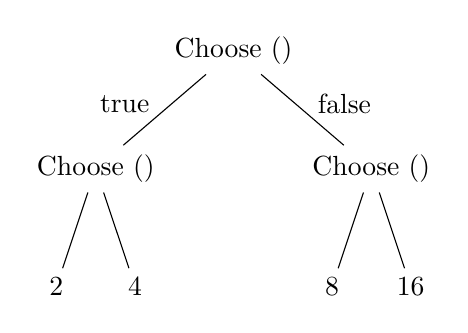
\begin{tikzpicture}[level distance=1.5cm,
level 1/.style={sibling distance=3.5cm},
level 2/.style={sibling distance=1cm}]
%\tikzstyle{every node}=[circle,draw]

\node (Root) [draw=none,rectangle] {Choose ()}
    child { node[draw=none] (q0) {Choose ()} 
      child { node[draw=none] (q00) {2}
      }
      child { node[draw=none] (q01) {4} 
      }
      edge from parent node [draw=none,left,xshift=-2.0,yshift=2.0] {true}
    }
    child { node [draw=none] (q1) {Choose ()}
      child { node[draw=none] (q10) {8}
      }
      child { node[draw=none] (q11) {16}       
      }
      edge from parent node [draw=none,right,xshift=2.0,yshift=2.0] {false}
    };
\end{tikzpicture}
\end{center}\caption{Interpretation of the conditional expression as a computation tree. The left edges correspond to taking the first branch in a conditional expression. Analogously, the right edges correspond to taking the second branch.}\label{fig:condexp}
\end{figure}
During evaluation of the expression we eventually have to interpret the root node \type{Choose} in Figure \ref{fig:condexp} and possibly its immediate subtrees.
There are multiple possible interpretations. One interpretation is to always interpret \type{Choose} as \code{true} which figuratively corresponds to taking the left (true) branch. The node we arrive at is also a \type{Choose}-node, so again we choose the left branch arriving at a leaf that contains the concrete value $2$. Hence under this interpretation the handler collapses the computation tree to the leaf $2$. Dually, we could always choose false which leads to the output value $16$. Figures \ref{fig:positive} and \ref{fig:negative} illustrate the two interpretation respectively.
\begin{figure*}[t!]
    \centering
    \begin{subfigure}[t]{0.5\textwidth}
        \centering
\begin{tikzpicture}[level distance=1.5cm,
level 1/.style={sibling distance=3.5cm},
level 2/.style={sibling distance=1cm}]
%\tikzstyle{every node}=[circle,draw]

\node (Root) [draw=none,rectangle] {Choose ()}
    child { node[draw=none] (q0) {Choose ()} 
      child { node[draw=none] (q00) {2}
      }
      child { node[draw=none] (q01) {4} 
      }
      edge from parent node [draw=none,left,xshift=-2.0,yshift=2.0] {true}
    }
    child { node [draw=none] (q1) {Choose ()}
      child { node[draw=none] (q10) {8}
      }
      child { node[draw=none] (q11) {16}       
      }
      edge from parent node [draw=none,right,xshift=2.0,yshift=2.0] {false}
    };
\draw[->,black,rounded corners,dashed,line width=0.7pt]
     ($(Root) +(-1.0,0.2)$) --
     ($(q0) +(-1.0,0.4)$) --
     ($(q00) +(-0.3,0.0)$);
\end{tikzpicture}
        \caption{The ``positive'' interpretation: Always choose true. Output: 2.}\label{fig:positive}
    \end{subfigure}%
    ~ 
    \begin{subfigure}[t]{0.5\linewidth}
        \centering
 \begin{tikzpicture}[level distance=1.5cm,
level 1/.style={sibling distance=3.5cm},
level 2/.style={sibling distance=1cm}]
%\tikzstyle{every node}=[circle,draw]

\node (Root) [draw=none,rectangle] {Choose ()}
    child { node[draw=none] (q0) {Choose ()} 
      child { node[draw=none] (q00) {2}
      }
      child { node[draw=none] (q01) {4} 
      }
      edge from parent node [draw=none,left,xshift=-2.0,yshift=2.0] {true}
    }
    child { node [draw=none] (q1) {Choose ()}
      child { node[draw=none] (q10) {8}
      }
      child { node[draw=none] (q11) {16}       
      }
      edge from parent node [draw=none,right,xshift=2.0,yshift=2.0] {false}
    };
\draw[->,black,rounded corners,dashed,line width=0.7pt]
     ($(Root) +(1.0,0.2)$) --
     ($(q1) +(1.0,0.4)$) --
     ($(q10) +(1.3,0.0)$);
\end{tikzpicture}
        \caption{The ``negative'' interpretation: Always choose false. Output: 16.}\label{fig:negative}
    \end{subfigure}    
\end{figure*}
Alternatively, we could make a random choice between true and false at each branch. Again, this interpretation leads to one single output value. Albeit, the output value would be non-deterministic under this interpretation. 

Yet another interpretation is to enumerate all possible choices. For example, we can choose explore the left branch and thereafter the right branch at each node. Under this interpretation we effectively visit the entire tree. Therefore, the handler transforms the computation tree into a set of its leaves. Figure \ref{fig:enumerate} illustrates the tree traversal.
\begin{figure}[H]
\begin{center}
\begin{tikzpicture}[level distance=1.5cm,
level 1/.style={sibling distance=3.5cm},
level 2/.style={sibling distance=1cm}]
%\tikzstyle{every node}=[circle,draw]
\node (Root) [draw=none,rectangle] {Choose ()}
    child { node[draw=none] (q0) {Choose ()} 
      child { node[draw=none] (q00) {2}
      }
      child { node[draw=none] (q01) {4} 
      }
      edge from parent node [draw=none,left,xshift=-2.0,yshift=2.0] {true}
    }
    child { node [draw=none] (q1) {Choose ()}
      child { node[draw=none] (q10) {8}
      }
      child { node[draw=none] (q11) {16}       
      }
      edge from parent node [draw=none,right,xshift=2.0,yshift=2.0] {false}
    };
\draw[->,black,rounded corners,dashed,line width=0.7pt]
     ($(Root) +(-1.0,0.2)$) --
     ($(q0) +(-1.0,0.4)$) --
     ($(q00)  +(-0.5,0.0)$) --
     ($(q00)  +(-0.4,-0.35)$) --
     ($(q00)  +(0.0,-0.5)$) --
     ($(q00)  +(0.4,-0.35)$) --
     ($(q00)  +(0.5,0.0)$) --
     ($(q0)  +(-0.005,-0.3)$) --
     ($(q01)  +(-0.35,-0.35)$) --
     ($(q01)  +(0.0,-0.45)$) --
     ($(q01)  +(0.35,-0.35)$) --
     ($(q01)  +(0.4,0.0)$) --
     ($(q0)   +(1.0,0.5)$) --
     ($(Root) +(-0.3,-0.4)$) --
     ($(q1)  +(-0.8,-0.1)$) --
     ($(q10)  +(-0.5,0.0)$) --
     ($(q10)  +(-0.4,-0.35)$) --
     ($(q10)  +(0.0,-0.5)$) --
     ($(q10)  +(0.4,-0.35)$) --
     ($(q10)  +(0.5,0.0)$) --
     ($(q1)  +(-0.005,-0.3)$) --
     ($(q11)  +(-0.35,-0.35)$) --
     ($(q11)  +(0.0,-0.45)$) --
     ($(q11)  +(0.35,-0.35)$) --
     ($(q11)  +(0.4,0.0)$);
\end{tikzpicture}\caption{Enumerate all possible choices. Output: $\{2,4,8,16\}$.}\label{fig:enumerate}
\end{center}
\end{figure}
The interpretations we have discussed so far share a characteristic: Each node (operation) is handled uniformly. That is, the same strategy is applied to similar nodes. This holds in general for any handler and computation. So, we can think of handlers as kinds of fold-functions that transform computation trees \cite{Kammar2013}.